% Massimo Zannoni - Curriculum Vitae
%
% This work is licensed under a Creative Commons Attribution-ShareAlike 4.0 International License (CC BY-SA 4.0)

\documentclass[a4paper]{article}
\usepackage{graphicx}
\usepackage[top=2.4cm, bottom=2.4cm, left=2cm, right=2cm]{geometry}
\usepackage[utf8]{inputenc}
\usepackage{hyperref}
\usepackage[english]{babel}

%% set the font family
\usepackage[condensed,math]{kurier}
%% set the font encoding
\usepackage[T1]{fontenc}
%% details about the font
%% https://ctan.org/tex-archive/fonts/kurier/

%\usepackage{mdwlist} % needed for itemize*
%\usepackage{tabu} % package for advanced table features
\usepackage{longtable}
\usepackage{array}

\usepackage{enumitem}
%next line to avoid vertical separation before an itemize section
%\setlist{nolistsep}

% Personal details
\def\nome{Massimo Zannoni}
\def\email{myemail@someservice.abc}
\def\telefono{+00 11 22 33 44}
\def\nazionalita{Italian}
\def\datadinascita{00.00.1900}
\def\genere{he\,/\,him}
\def\indirizzo{Squarestreet, 1 \newline 0000 Zürich \newline CH}
\def\sito{https://www.fotobill.com}

% Web links and logos
\def\githublink{https://github.com/mzannoni}
\def\gitlablink{https://gitlab.com/mzannoni}
\def\linkedinlink{https://www.linkedin.com/in/mzannoni}
\def\githublogo{pics/github-mark/github-mark.png}
\def\gitlablogo{pics/gitlab-logo/gitlab-logo-600.png}
\def\linkedinlogo{pics/linkedin-logo/LI-In-Bug-black.png}

% Define some lengths used in the document
\newlength{\sectsep}
\setlength{\sectsep}{0.6cm}
\newlength{\subsectsep}
\setlength{\subsectsep}{0.4cm}
\newlength{\detsep}
\setlength{\detsep}{0.4cm}

% Edit PDF file properties
\hypersetup{
  pdfauthor = {\nome},
  pdfcreator = {\nome},
  pdfkeywords = {electronics, IC design, RF measurement, optoelectronics, image sensors, engineering},
  pdftitle = {\nome ~- Curriculum Vitae},
  pdfsubject = {Curriculum Vitae},
  % next line to avoid links from being blue and underlined
  hidelinks
}

% Format two pieces of text, one left aligned and one right aligned
\newcommand{\headerrow}[2]
{\begin{tabular*}{\textwidth}{l@{\extracolsep{\fill}}r}
	#1 &
	#2 \\
\end{tabular*}}

% Make lists with diamonds and compact spacing
\renewenvironment{itemize}{
  \begin{list}{$\diamond$}{
    \setlength{\topsep}{0.25em}
    \setlength{\itemsep}{0em}
    \setlength{\parskip}{0pt}
    \setlength{\parsep}{0em}
  }
}{
  \end{list}
}

% Make lists with small dots and compact spacing
\newenvironment{itemize2}{
  \begin{list}{$\cdot$}{
    \setlength{\topsep}{0.25em}
    \setlength{\itemsep}{0em}
    \setlength{\parskip}{0pt}
    \setlength{\parsep}{0em}
  }
}{
  \end{list}
}

\begin{document}
  \begin{longtable}{r || l}

  % 1st row: Title, details and photo
  \hfill
  & \begin{minipage}{0.5\textwidth}
      \vspace{0.2\sectsep}
      \section*{\nome}
      \vspace{\detsep}
      \indirizzo \vspace{\detsep} \\
      \href{mailto:\email}{\email} ~|~ \telefono \vspace{\detsep} \\
      \datadinascita ~|~ \nazionalita ~|~ \genere \vspace{\detsep} \\
      %\datadinascita ~|~ \nazionalita \vspace{\detsep} \\
    \end{minipage}
    %\hfill
    \begin{minipage}{0.3\textwidth}
      \vspace{0.4cm}
      {\centering
      	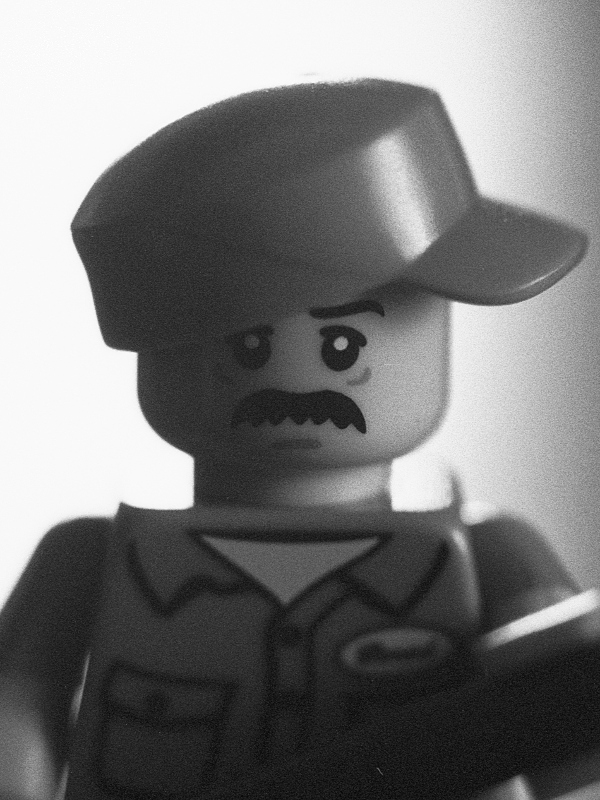
\includegraphics[width=0.5\textwidth]{pics/portrait} \vspace{0.1cm} \\
      	% raisebox is used to center the logos vertically
      	\raisebox{-0.5\height}{\href{\githublink}{\includegraphics[height=3.2ex]{\githublogo}}}
      	~
      	\raisebox{-0.5\height}{\href{\gitlablink}{\includegraphics[height=4ex]{\gitlablogo}}}
      	~
      	\raisebox{-0.5\height}{\href{\linkedinlink}{\includegraphics[height=3.2ex]{\linkedinlogo}}}
      	\vspace{0.1cm}
      	\\
      }
    \end{minipage} \\
  \hline \hline

  %2nd row: Working experience 1
  & \begin{minipage}{0.9\textwidth}
      \vspace{\sectsep}
      \subsection*{Working Experience}
      \subsubsection*{Senior Analog Design Engineer}
      \headerrow
  		{\textbf{Sony AVS AG} (formerly Insightness AG)}{\emph{2017 - current}}
      \\
      \headerrow
        {\emph{Wiesenstrasse 5, 8952 Schlieren, CH}}{}
      \\
      \headerrow
        {Image Sensors / Computer Vision}{}

      \begin{itemize}
          \item Analog IC design in CMOS technology
          \begin{itemize2}
              \item Event-Based Image Sensor
              \item 3D-IC
          \end{itemize2}
          \item Project leading for IC design
          \item Optical and electrical characterization
          \item IT and network infrastructure maintenance
      \end{itemize}
  \end{minipage} \\[\sectsep]

  %3rd row: Working experience 2
  & \begin{minipage}{0.9\textwidth}
      \vspace{\subsectsep}
      \subsubsection*{Design Engineer}
      \headerrow
  		{\textbf{GigOptix-Helix AG} (subsidiary of GigPeak, Inc.; now Renesas Electronics Corporation)}{\emph{2013 - 2017}}
      \\
      \headerrow
        {\emph{Seefeldstrasse 45, 8008 Zürich, CH}}{}
      \\
      \headerrow
        {Opto-electronics}{}

      \begin{itemize}
          \item High-speed analog IC design in BiCMOS technology
          \begin{itemize2}
              \item 28 Gbit/s TIA receivers and VCSEL drivers
          \end{itemize2}
          \item RF and optical measurement
          \item Customer support, production support and RMA analysis
      \end{itemize}
  \end{minipage} \\[\sectsep]

  %4th row: Working experience 3
  & \begin{minipage}{0.9\textwidth}
      \vspace{\sectsep}
      \subsubsection*{Thesis Worker}
      \headerrow
  		{\textbf{ABB AB Corporate Research Center}}{\emph{July 2012 - December 2012}}
      \\
      \headerrow
        {\emph{Forskargränd 7, 722 26 Västerås, Sweden}}{}
      \\
      \headerrow
          {Power Technology Dept., Electric Power System Group}{}

      \begin{itemize}
          \item Semiconductor device modeling
          \item Power Electronics
      \end{itemize}
  \end{minipage} \\[\sectsep]

  %5th row: Education 1
  & \begin{minipage}{0.9\textwidth}
      \vspace{\sectsep}
      \subsection*{Education}
      \subsubsection*{MSc in Electronic Engineering}
      \headerrow
  		{\textbf{Università degli Studi di Parma, Italy}}{\emph{2009 - 2013}}
      \\
      \headerrow
        {\emph{Faculty of Engineering}}{}
      \\
      \headerrow
        {Analog/Digital IC Design, Semiconductor Physics, Sensor Technology, Power Electronics}{}

      \begin{itemize}
          \item Thesis: \emph{PSpice Modeling of 4.5 kV StakPak\textsuperscript{TM} Modules}
          \item Grade: 107/110
      \end{itemize}
      \vfill
  \end{minipage} \\[\sectsep]

  %6th row: Education 2
  & \begin{minipage}{0.9\textwidth}
      \vspace{\subsectsep}
      \subsubsection*{BSc in Electronic Engineering}
      \headerrow
  		{\textbf{Università degli Studi di Parma, Italy}}{\emph{2005 - 2009}}
      \\
      \headerrow
        {\emph{Faculty of Engineering}}{}
      \\
      \headerrow
        {Electronics, Electrotechnics, Information Technology, Controls, PCB Design}{}

      \begin{itemize}
          \item Thesis: \emph{Experimental Characterization of a Magneto-hydrodynamic Micro-Stirrer}
          \item Grade: 108/110
      \end{itemize}
      \vfill
  \end{minipage} \\[\sectsep]

  %7th row: Personal skills and competences
  & \begin{minipage}{0.9\textwidth}
      \vspace{\sectsep}
      \subsection*{Skills and Competences}
      \subsubsection*{Languages}
      \begin{tabular}{rl}
        \textbf{Italian:}&Native\\
        \textbf{English:}&Fluent\\
        \textbf{German:}&Beginner/Intermediate\\
      \end{tabular} \vspace{1.5ex} \\
      %\hspace*{0.5em} {\footnotesize \emph{See Common European Framework (CEF) self-assessment table in the appendix.}}
    \end{minipage} \\[\sectsep]

  %8th row: Technical skills and competences
  & \begin{minipage}{0.9\textwidth}
      \vspace{\subsectsep}
      \subsubsection*{Technical and Organizational}
      \begin{itemize}
          \item Analog IC Design
          \item 3D-IC
          \item Project leading and work coordination
          \item Full-custom analog IC layout
          \item Electrical and optical measurements and characterization
          \item Effective problem-solving approach in non-standard context
          \item Data analysis and elaboration
          \item Frequently switch between different kinds of task
          \item Explain design issues across technical domains
      \end{itemize}
  \end{minipage} \\[\sectsep]

  %9th row: Computer skills and competences
  & \begin{minipage}{0.9\textwidth}
      \vspace{\subsectsep}
      \subsubsection*{Computer Tools and Software Development}
      \begin{tabular*}{\textwidth}{r p{0.75\textwidth}}
        Operating Systems:&{Linux: very good knowledge\newline Microsoft Windows: good knowledge}\\[0.5ex]
        Electronic CAD:&Cadence DFII (Virtuoso, Spectre), Mentor TannerTools, Mentor Calibre, Mentor AFS, SPICE, Cadence OrCAD (PSpice)\\[0.5ex]
        Programming:&Python, C/C++, Matlab/Octave, shell scripting, VHDL, Verilog/VerilogA, {\fontfamily{arial}\selectfont\LaTeX}\\[0.5ex]
        Version Control:&Git, Subversion, ClioSoft SOS
      \end{tabular*}\\
  \end{minipage} \\[\sectsep]

  %10th row: Other skills and competences
  & \begin{minipage}{0.9\textwidth}
      \vspace{\subsectsep}
      \subsubsection*{Others}
      \begin{itemize}
          \item Good photo-editing and computer drawing skills
          \item Hand-working: good familiarity with tools and instruments for building electronic systems; basic skills in the use of main mechanic hand-tools and power-tools
      \end{itemize}
  \end{minipage} \\[\sectsep]

  %11th row: Personal Interests
  & \begin{minipage}{0.9\textwidth}
      \vspace{\subsectsep}
      \subsubsection*{Personal Interests}
      \begin{itemize}
          \item Photography
          \item Love for traveling
          \item Archery
          \item Love for the mountains (particularly, hiking and MTB)
      \end{itemize}
  \end{minipage} \\[\sectsep]

  %12th row: Annexes
  & \begin{minipage}{0.9\textwidth}
      \vspace{\subsectsep}
      \subsubsection*{Annexes}
      \begin{itemize}
          \item Appendix including patents, publications and references
          \item Reference letters (\emph{Arbeitszeugnisse}) by former managers available upon request
          \item Personal website: \href{\sito}{\sito}
      \end{itemize}
      \vfill
    \end{minipage} \\

  \end{longtable}
\end{document}
